\section{Factorized Higher-Order IVM}
\label{sec:factorized_IVM}

We introduce incremental view maintenance in our factorized ring computation framework. In contrast to evaluation, the incremental maintenance of the query result may require the materialization and maintenance of views. An update to a relation $\VIEW{R}$ triggers changes in all views from the leaf $\VIEW{R}$ to the root of the view tree. 


\paragraph{\textbf{Updates.}}
The insertion (deletion) of a tuple $\textvec{t}$ into (from) a relation $\VIEW{R}$ is expressed as a delta relation $\delta\VIEW{R}$ that maps $\textvec{t}$ to $\RINGONE$ (and respectively $-\RINGONE$). In general, $\delta\VIEW{R}$ can be a relation, thus a collection of tuples mapped to payloads. The updated relation is then the union of the old relation and the delta relation: $\VIEW{R} := \VIEW{R} \VPLUS \delta\VIEW{R}$. 


\paragraph{\textbf{Delta Views.}}
For each view $\VIEW{V}$ affected by an update, a {\em delta view} $\VIEW{\delta{V}}$ defines the change in the view content. In case the view $\VIEW{V}$ represents a relation $\VIEW{R}$, then $\VIEW{\delta{V}}=\VIEW{\delta{R}}$ if there are updates to $\VIEW{R}$ and  $\VIEW{\delta{V}}=\emptyset$ otherwise. If the view is defined using operators on other views, $\delta\VIEW{V}$ is derived using the following delta rules:
% 
\begin{align*}
  \quad
  \delta{(\VIEW{V_1} \VPLUS \VIEW{V_2})} &= \delta{\VIEW{V_1}} \VPLUS \delta{\VIEW{V_2}} \\
  \nop{\delta{(-\VIEW{V_1})} &= -\delta{\VIEW{V_1}} \\}
  \delta{(\VIEW{V_1} \VPROD \VIEW{V_2})} &= (\delta{\VIEW{V_1}} \VPROD \VIEW{V_2}) \VPLUS (\VIEW{V_1} \VPROD\delta{\VIEW{V_2}}) \VPLUS (\delta{\VIEW{V_1}} \VPROD \delta{\VIEW{V_2}})\\
  \delta{(\VSUM_{X}\VIEW{V})} &= \VSUM_{X}\delta{\VIEW{V}}
\end{align*}

The correctness of the rules follows from the associativity of $\VPLUS$ and the distributivity of $\VPROD$ over $\VPLUS$; $\VSUM_{X}$ is equivalent to the repeated application of $\VPLUS$ for the possible values of $X$. The derived delta views are subject to standard simplifications: If $\VIEW{V}$ is not defined over the updated relation $\VIEW{R}$, then its delta view $\VIEW{\delta{V}}$ is empty, and then we propagate this information using the identities $\emptyset \VPLUS \VIEW{V} = \VIEW{V} \VPLUS \emptyset = \VIEW{V}$ and $\emptyset \VPROD \VIEW{V} = \VIEW{V} \VPROD \emptyset = \emptyset$.


\medskip

\begin{figure}[t]
\centering
\setlength{\tabcolsep}{3pt}
%
\begin{tabular}{@{}c@{}c@{~~~~}l@{}}
    \toprule
    \multicolumn{3}{c}{$\Delta$(\text{view tree} $\tau$, \text{update} $\VIEW{\delta{R}}$) : delta view tree}\\
    \midrule
    \multicolumn{3}{l}{\MATCH $\tau$:}\\
    \midrule
    \phantom{a} & $\VIEW{R}[\mathit{\sch(\VIEW{R})}]$ & \hspace*{-0.5em}\RETURN $\VIEW{\delta{R}}[\mathit{\sch(\VIEW{R})}]$\\[2pt]
    \cmidrule{2-3} \\[-6pt]
    &    
    \begin{minipage}[t]{1.6cm}
        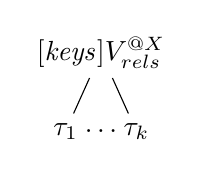
\begin{tikzpicture}[xscale=0.45, yscale=1]
            \node at (0,-2)  (n4) {$\VIEW[{\it keys}]{V^{@X}_{rels}}$};
            \node at (-1,-3)  (n1) {$\tau_1$} edge[-] (n4);
            \node at (0,-3)  (n2) {$\ldots$};
            \node at (1,-3)  (n3) {$\tau_k$} edge[-] (n4);
        \end{tikzpicture}        
    \end{minipage}
    &
    \begin{minipage}[t]{8.2cm}
\vspace{-4.5em}
 \hspace*{-0.5em}\LET $\VIEW[{\it keys_i}]{V^{@X_i}_{rels_i}}\text{ be root of } \tau_i, \ \forall i\in[k]$\\[0.5ex]
\hspace*{-0.5em}\LET $j\in[k] \text{ be such that } \VIEW{R}\in\mathsf{rels}_j$ \\[0.5ex]    
\hspace*{-0.5em}\LET $\delta\VIEW[\mathit{keys}]{V}  = \delta\VIEW[{\it keys_j}]{V_{rels_j}^{@X_j}} \underset{i\in[k],i\neq j}{\VPRODBIG}\!\VIEW[{\it keys_i}]{V^{@X_i}_{rels_i}}$\\[0.5ex]
\IF $X \notin {\it keys}$ \\[0.5ex]   
\TAB $\delta\VIEW[\mathit{keys}]{V^{@X}_{rels}}  = \textsc{Optimize}\big( \VSUM_{X} \delta\VIEW[{\it keys}]{V} \, \big)$\\[0.5ex]
\ELSE \\[0.5ex]   
\TAB $\delta\VIEW[\mathit{keys}]{V^{@X}_{rels}}  = \delta\VIEW[{\it keys}]{V}$\\[0.5ex]
        \RETURN $
				\left\{
				\begin{array}{@{~~}c@{~~}}
					\tikz {
				\node at (1,-1)  (n4) {$\VIEW[\mathit{keys}]{V^{@X}_{rels}}$};
				\node at (-0.8,-1.75)  (n1) {$\tau_1$} edge[-] (n4);
				\node at (-0.1,-1.75)  (n2) {$\ldots$};
				\node at (1,-1.75)  (n3) {$\Delta(\tau_j, \delta \VIEW{R})$} edge[-] (n4);
				\node at (2,-1.75)  (n2) {$\ldots$};
				\node at (2.8,-1.75)  (n3) {$\tau_k$} edge[-] (n4);
					}
				\end{array}  \right.$
    \end{minipage}
    \\
    \bottomrule
\end{tabular}
\caption{Creating a delta view tree $\Delta(\tau,\VIEW{\delta{R}})$ for a view tree $\tau$ to process an update $\VIEW{\delta{R}}$ to relation $\VIEW{R}$. }
\label{fig:dynamic_view_tree_algo}
\end{figure}

\paragraph{\textbf{Delta Trees.}}
Under updates to one relation, a view tree becomes a delta tree where the affected views become delta views. The function $\Delta$ in Figure~\ref{fig:dynamic_view_tree_algo} 
replaces the views along the path from the updated relation to the root with delta views.
The {\sc Optimize} method rewrites delta view expressions to exploit factorized updates by avoiding the materialization of Cartesian products and pushing marginalization past joins; we explain this optimization in Section~\ref{sec:factorizable_updates}.

\begin{example}
\label{ex:delta_view_tree}
Consider again the query from Example~\ref{ex:sql_count}, its view tree in Figure~\ref{fig:example_payloads}, and the same relations over the $\mathbb{Z}$ ring 
and the lifting functions that map all values to $1$ as in Example~\ref{ex:views_count}. 
%
An update $\VIEW{\delta{T}}[C,D]=\{ \tuple{c_1,d_1} \to -1, \tuple{c_2, d_2} \to 3 \}$ triggers 
delta computation at each view from the leaf $\VIEW{T}$ to the root of the view tree:
\begin{align*}
  \qquad
  \delta\VIEW[C]{V^{@D}_{T}} &= \VSUM_{D} \delta\VIEW[C,D]{T} \\
  \delta\VIEW[A]{V^{@C}_{ST}} &= \VSUM_{C} \delta\VIEW[C]{V^{@D}_{T}} \VPROD \VIEW[A,C]{V^{@E}_{S}} \\
  \delta\VIEW[~]{V^{@A}_{RST}} &= \VSUM_{A} \VIEW[A]{V^{@B}_{R}} \VPROD \delta\VIEW[A]{V^{@C}_{ST}}
\end{align*}
%
%
%Given the contents of $\VIEW{V^{@E}_{S}}$ and $\VIEW{V^{@B}_{R}}$ from Example~\ref{ex:views_count},  
%we now have:

Given that $\VIEW{V^{@E}_{S}} =$ 
$\{(a_1,c_1) \to 2,$ $(a_1,c_2) \to 1,$ $(a_2,c_2) \to 1\}$ 
and $\VIEW{V^{@B}_{R}} =$ 
$\{a_1 \to 2,$ $a_2 \to 1,$ $a_3 \to 1\}$,
we obtain
 $\delta\VIEW{V^{@D}_{T}}[C] = \{c_1 \to -1,$ $c_2 \to 3\}$, 
 $\delta\VIEW{V^{@C}_{ST}}[A] = \{a_1 \to 1,$ $a_2 \to 3\}$, and 
 $\delta\VIEW{V^{@A}_{RST}} = \{() \to 5\}$. 
  
 \nop{
\begin{center}
\begin{tabular}{@{}ccc@{}}
  \begin{tabular}[t]{@{}l@{~$\to$~}l}
  C & $\delta\VIEW{V^{@D}_{T}}[C]$  \\\toprule
  $c_1$ & $-1$ \\
  $c_2$ & $3$
  \end{tabular}
  &
  \begin{tabular}[t]{@{}l@{~$\to$~}l}
  A & $\delta\VIEW{V^{@C}_{ST}}[A]$\\\toprule
  $a_1$ & $1$ \\
  $a_2$ & $3$
  \end{tabular}
  &
  \begin{tabular}[t]{@{}l@{~$\to$~}l}
  $()$ & $\delta\VIEW{V^{@A}_{RST}}$ \\\toprule
  $\tuple{}$ & $5$
  \end{tabular}
\end{tabular}
\end{center}
}
A single-tuple update to $\VIEW{T}$ fixes the values for $C$ and $D$. Computing $\delta\VIEW{V^{@D}_{T}}$ then takes constant time. The delta view $\delta\VIEW{V^{@C}_{ST}}$ iterates over all possible $A$-values for a fixed $C$-value, which takes linear time; $\delta\VIEW{V^{@A}_{RST}}$ incurs the same linear-time cost. A single-tuple update to $\VIEW{R}$ or $\VIEW{S}$
fixes all variables on a leaf-to-root path in the delta view tree, giving a constant view maintenance cost.
\punto
\end{example}

In contrast to classical (first-order) IVM that only requires maintenance of the query result~\cite{Chirkova:Views:2012:FTD}, our approach is higher-order IVM as updates may trigger ma\-intenance of several interrelated views. The fully-recur\-sive IVM scheme of DBToaster~\cite{Koch:Ring:2010:PODS,DBT:VLDBJ:2014} creates one materialization hierarchy per relation in the query, whereas we use one view tree for all relations. This view tree relies on variable orders to decompose the query into views and factorize its computation and maintenance.

\paragraph{\textbf{Which Views to Materialize and Maintain?}}
The answer to this question depends on which relations may change. 
The set of the updatable relations determines the possible delta propagation paths in a view tree, and these paths may use materialized views.
% Let $\mathcal{U}$ be the set of the updatable relations. 
% This set determines the possible delta propagation paths in a view tree.

\begin{figure}[t]
\centering
\setlength{\tabcolsep}{3pt}
%
\begin{tabular}[t]{@{}c@{}c@{~~~}l}
    \toprule
    \multicolumn{3}{c}{$\mu$(\text{view tree} $\tau$, \text{updatable relations} $\mathcal{U}$) : view set}\\
    \midrule
    \multicolumn{3}{l}{\MATCH $\tau$:}\\
    \midrule 
    \phantom{ab}
    &
    \hspace{-4mm}
    \begin{minipage}[t]{1.5cm}
        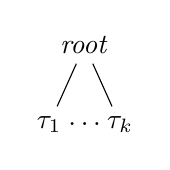
\begin{tikzpicture}[xscale=0.45, yscale=1]
            \node at (0,-2)  (n4) {$\mathit{root}$};
            \node at (-1,-3)  (n1) {$\tau_1$} edge[-] (n4);
            \node at (0,-3)  (n2) {$\ldots$};
            \node at (1,-3)  (n3) {$\tau_k$} edge[-] (n4);
        \end{tikzpicture}
    \end{minipage}
    &
    \begin{minipage}[t]{8.55cm}
        \vspace{-4em}
        $\mathit{children} = \{ \VIEW{V_i} \text{ is root of } \tau_i \}_{i\in[k]}$\\[0.5ex]
        $\mathit{m\_root} = \IF\SPACE (\mathit{root} \,\text{ has no parent})\SPACE \{ \VIEW{\mathit{root}} \} \SPACE\ELSE\SPACE \emptyset$\\[0.5ex]
        $\mathit{m\_children} = 
          \{ \VIEW{V_i} \mid \VIEW{V_i}, \VIEW{V_j} \in \mathit{children}, $\\[0.5ex]
        $\TAB\TAB\TAB\TAB\TAB\TAB\TAB\SPACE \VIEW{V_i} \neq \VIEW{V_j}, \mathsf{rels}(\VIEW{V_j}) \cap \mathcal{U} \neq \emptyset \}$\\[0.5ex]
        $\RETURN\SPACE \mathit{m\_root} \,\cup\, \mathit{m\_children} \,\cup\, \bigcup_{i\in[k]} \mu(\tau_i, \mathcal{U})$
    \end{minipage}\\
    \bottomrule
\end{tabular}
\caption{Deciding which views in a view tree $\tau$ to materialize in order to support updates to a set of relations $\mathcal{U}$. The notation $\mathsf{rels}(\VIEW{V_j})$ denotes the relations under the view $\VIEW{V_j}$ in $\tau$.}
\label{fig:materialization_view_tree_algo}
\end{figure}

Propagating changes along a leaf-to-root path is co\-mputationally most effective if each delta view joins with sibling views that are already materialized. 
Figure~\ref{fig:materialization_view_tree_algo} gives an algorithm that reflects this idea: Given a view tree $\tau$ and a set of updatable relations $\mathcal{U}$, the algorithm traverses the tree top-down to discover the views that need to be materialized. The root of the view tree $\tau$ is always stored as it represents the query result. Every other view $\VIEW{V_i}$ is stored only if there exists a sibling view $\VIEW{V_j}$ defined over an updatable relation. The algorithm returns the set of chosen views.


\nop{
Figure~\ref{fig:materialization_view_tree_algo} depicts an algorithm that reflects this idea: Given a view tree $\tau$ and a set of updatable relations $\mathcal{U}$, the algorithm builds a {\em materialization tree} $\mu(\tau, \mathcal{U})$ that has the same structure as $\tau$ and where each node is a Boolean value indicating whether the corresponding view from $\tau$ should be materialized. The root view is always stored as it represents the query result, that is, it has no parent: $\VIEW{par}=\mathit{null}$; every other view $\VIEW{V}$ is stored only if it is used to compute the delta of its parent for updates to a relation over which $\VIEW{V}$ is not defined, that is, there are updatable relations for the parent and not for $\VIEW{V}$ itself: $(\VIEW{rels(par)} \setminus \VIEW{rels}) \cap \mathcal{U} \neq \emptyset$. 
}

\begin{example}
We continue with our query from Example~\ref{ex:delta_view_tree}. For updates to $\VIEW{T}$ only, that is, $\mathcal{U} = \{ \VIEW{T} \}$, we store the root $\VIEW{V^{@A}_{RST}}$ and the views $\VIEW{V^{@E}_{S}}$ and $\VIEW{V^{@B}_{R}}$ used to compute the deltas $\VIEW{\delta{V^{@C}_{ST}}}$ and $\VIEW{\delta{V^{@A}_{RST}}}$. Only the root view is affected by these changes and maintained as: 
\begin{align*}
  \qquad
  \VIEW[~]{V^{@A}_{RST}} = \VIEW[~]{V^{@A}_{RST}} \VPLUS \VIEW[~]{\delta{V^{@A}_{RST}}}
\end{align*}
It is not necessary to maintain other views. If we would like to also support updates to $\VIEW{R}$ and $\VIEW{S}$, then we would also need to materialize $\VIEW{V^{@C}_{ST}}$ and $\VIEW{V^{@D}_{T}}$. 
If no updates are supported, then only the root view is stored. 
\punto
\end{example}

For queries with free variables, several views in their (delta) view trees may be identical: This can happen when all variables in their keys are free and thus cannot be marginalized. For instance, a variable order $\omega$ for the query from Example~\ref{ex:sql_sum_aggregate} may have the variables $A$ and $C$ above all other variables, in which case their views are the same in the view tree for $\omega$. We then store only the top view out of these identical views. 


\paragraph{\textbf{IVM Triggers.}}
For each updatable relation $\VIEW{R}$, our framework constructs a trigger procedure that takes as input an update $\VIEW{\delta{R}}$ and implements the maintenance schema of the corresponding delta view tree. This procedure also maintains all materialized views needed for the given update workload. 

A bulk of updates to several relations is handled as a sequence of updates, one per relation. Update sequences can also happen when updating a relation $\VIEW{R}$ that occurs several times in the query. The instances representing the same relation are at different leaves in the delta tree and lead to changes along multiple leaf-to-root paths. 